% ============================================================
%  PCD / MISS1202O2 – Concurrent and Distributed Programming
%  Homework 1 – Network Transfer Benchmark
%  Report document
% ============================================================
\documentclass[12pt,a4paper]{article}

% ── Packages ────────────────────────────────────────────────
\usepackage[T1]{fontenc}
\usepackage[utf8]{inputenc}
\usepackage[english]{babel}
\usepackage{geometry}
\geometry{margin=2.5cm}

\usepackage{graphicx}
\usepackage{booktabs}
\usepackage{longtable}
\usepackage{array}
\usepackage{multirow}
\usepackage{xcolor}
\usepackage{listings}
\usepackage{hyperref}
\usepackage{amsmath}
\usepackage{caption}
\usepackage{subcaption}
\usepackage{pgfplots}
\pgfplotsset{compat=1.18}
\usepackage{float}
\usepackage{enumitem}
\usepackage{fancyhdr}
\usepackage{titlesec}
\usepackage{microtype}

% ── Listing style ────────────────────────────────────────────
\lstset{
  language=bash,
  basicstyle=\ttfamily\small,
  keywordstyle=\color{blue},
  commentstyle=\color{gray},
  stringstyle=\color{red!70!black},
  breaklines=true,
  frame=single,
  backgroundcolor=\color{gray!8},
  numbers=none,
  xleftmargin=5pt,
  xrightmargin=5pt,
}

% ── Header / Footer ──────────────────────────────────────────
\pagestyle{fancy}
\fancyhf{}
\lhead{\small PCD / MISS1202O2 -- Homework 1}
\rhead{\small Network Transfer Benchmark}
\cfoot{\thepage}

% ── Hyperref ─────────────────────────────────────────────────
\hypersetup{
  colorlinks=true,
  linkcolor=blue!70!black,
  urlcolor=blue!70!black,
  citecolor=blue!70!black,
}

% ── Custom colours ───────────────────────────────────────────
\definecolor{tcpblue}{RGB}{41,128,185}
\definecolor{udporange}{RGB}{230,126,34}
\definecolor{quicgreen}{RGB}{39,174,96}

% ============================================================
\begin{document}

% ── Title page ───────────────────────────────────────────────
\begin{titlepage}
  \centering
  \vspace*{2cm}
  {\LARGE\bfseries Faculty of Automatic Control and Computers\\[0.4em]
   Politehnica University of Bucharest\par}
  \vspace{1.5cm}
  {\large\itshape MISS1202O2 – Concurrent and Distributed Programming\par}
  \vspace{2cm}
  \rule{\linewidth}{1pt}\\[0.6em]
  {\Huge\bfseries Homework 1\\[0.3em]
   Network Transfer Benchmark\\[0.3em]
   (TCP / UDP / QUIC)\par}
  \rule{\linewidth}{1pt}
  \vspace{2cm}
  {\large 2026\par}
  \vfill
  {\normalsize
   \textit{Tools used:} C~(C11), OpenSSL~3.x, POSIX sockets, GNU~Make\\[0.3em]
   \textit{Platform:} Linux (x86-64)}
\end{titlepage}

% ── Table of Contents ────────────────────────────────────────
\tableofcontents
\newpage

% ============================================================
\section{Introduction}
\label{sec:intro}

This report describes the design, implementation, and experimental evaluation
of a network data-transfer benchmark. The benchmark measures the time required
to transfer two representative data volumes (500\,MB and 1\,GB) over three
transport protocols---TCP, UDP, and QUIC---using two transfer modes
(\emph{streaming} and \emph{stop-and-wait}) and five block sizes ranging from
1\,B to 65\,535\,B.

The goal is to analyse the trade-offs between reliability, latency, and
throughput across different protocol and configuration combinations, and to
compare the built-in reliability of TCP with the application-level reliability
that must be added on top of UDP and QUIC.

% ============================================================
\section{System Architecture}
\label{sec:arch}

\subsection{File Structure}

\begin{description}[leftmargin=3cm, style=nextline]
  \item[\texttt{common.h}]  Shared wire-protocol definitions, data structures,
        SHA-256 helpers (via OpenSSL EVP), monotonic timer, and TCP
        send/recv helpers.
  \item[\texttt{client.c}]  Transfer-benchmark client; supports TCP, UDP, and
        QUIC protocols with streaming and stop-and-wait modes.
  \item[\texttt{server.c}]  Transfer-benchmark server; mirrors the client's
        protocol support and loops indefinitely accepting sessions.
  \item[\texttt{Makefile}]  Builds both binaries; also generates a self-signed
        TLS certificate (\texttt{server.cert} / \texttt{server.key}) required
        by QUIC.
\end{description}

\subsection{Wire Protocol}

All multi-byte integers are in big-endian (network) byte order.

\subsubsection{TCP and QUIC (stream-based)}

\begin{enumerate}
  \item Client $\to$ Server: \texttt{SessionHdr} (17\,B, sent once).
  \item Client $\to$ Server: \texttt{BlockHdr} (13\,B) $+$ payload (repeated).
  \item Server $\to$ Client: \texttt{Ack} (9\,B, stop-and-wait mode only,
        one per block).
\end{enumerate}

\subsubsection{UDP (datagram-based)}

\begin{enumerate}
  \item Client $\to$ Server: \texttt{UdpSessionPkt} (14\,B, session start).
  \item Server $\to$ Client: \texttt{UdpAckPkt} with \texttt{seq=UINT64\_MAX}
        (session confirmation).
  \item Client $\to$ Server: \texttt{UdpBlockHdr} (14\,B) $+$ payload
        (per datagram).
  \item Server $\to$ Client: \texttt{UdpAckPkt} (stop-and-wait mode only).
\end{enumerate}

\subsection{Data Integrity – SHA-256 Hashing}

Both the client and the server feed every payload byte into an OpenSSL
\texttt{EVP\_DigestUpdate} context. At the end of a session both sides print
the resulting SHA-256 hex digest. Matching digests confirm that the assembled
payload is identical on both ends.

The payload is generated deterministically: byte at offset $k$ equals
$k \bmod 256$, so no file I/O is required.

% ============================================================
\section{How to Build and Run}
\label{sec:usage}

\subsection{Prerequisites}

\begin{itemize}
  \item GCC $\geq$ 9 with C11 support.
  \item OpenSSL $\geq$ 3.2 with QUIC support
        (\texttt{libssl-dev}, \texttt{libcrypto}).
  \item GNU Make.
\end{itemize}

\subsection{Building}

\begin{lstlisting}
# From the homework1/ directory:
make
\end{lstlisting}

This compiles \texttt{client} and \texttt{server} and generates
\texttt{server.cert} / \texttt{server.key} (self-signed, valid for localhost).

\subsection{Server Usage}

\begin{lstlisting}
./server -p tcp|udp|quic  [-P PORT]  [-c CERT]  [-k KEY]

  -p  Protocol to listen on: tcp, udp, or quic      (required)
  -P  Port number                                    (default: 9999)
  -c  Path to TLS certificate PEM file               (QUIC only, default: server.cert)
  -k  Path to TLS private-key PEM file               (QUIC only, default: server.key)
\end{lstlisting}

The server loops indefinitely, printing session statistics after each
client disconnects. Stop it with \texttt{Ctrl-C}.

\subsection{Client Usage}

\begin{lstlisting}
./client -p tcp|udp|quic  -b BLOCK_SIZE  -d DATA_MB  [-H HOST]  [-P PORT]  [-m MODE]

  -p  Protocol: tcp, udp, or quic                   (required)
  -b  Block (message) size in bytes, 1..65535        (required)
  -d  Amount of data to transfer in MB               (required)
  -H  Server hostname or IP address                  (default: 127.0.0.1)
  -P  Port number                                    (default: 9999)
  -m  Transfer mode: streaming or stop-wait          (default: streaming)
\end{lstlisting}

\subsection{Example Sessions}

\paragraph{TCP – Streaming, 500\,MB, 1\,000\,B blocks}
\begin{lstlisting}
# Terminal 1 (server)
./server -p tcp

# Terminal 2 (client)
./client -p tcp -b 1000 -d 500
\end{lstlisting}

\paragraph{UDP – Stop-and-Wait, 500\,MB, 10\,000\,B blocks}
\begin{lstlisting}
./server -p udp
./client -p udp -b 10000 -d 500 -m stop-wait
\end{lstlisting}

\paragraph{QUIC – Streaming, 1\,GB, 65\,535\,B blocks}
\begin{lstlisting}
./server -p quic
./client -p quic -b 65535 -d 1024
\end{lstlisting}

\paragraph{Remote host}
\begin{lstlisting}
./server -p tcp -P 8080
./client -p tcp -H 192.168.1.10 -P 8080 -b 10000 -d 500
\end{lstlisting}

% ============================================================
\section{Implementation Details}
\label{sec:impl}

\subsection{TCP}

TCP is implemented using POSIX stream sockets (\texttt{SOCK\_STREAM}).  A
single \texttt{SessionHdr} is sent at connection time; each block is
prefixed with a \texttt{BlockHdr} carrying a 64-bit sequence number, the
actual payload size, and an \texttt{is\_last} flag.

\texttt{send\_all} / \texttt{recv\_all} wrappers loop over the underlying
\texttt{send}/\texttt{recv} calls to guarantee complete delivery of each
structure, because TCP is a byte stream and may deliver data in arbitrary
chunks.

In stop-and-wait mode the client waits for a 9-byte \texttt{Ack} from the
server before advancing to the next block. For TCP this adds latency with
no reliability benefit (TCP already handles retransmissions), but it is
included for comparative measurement.

\subsection{UDP}

UDP uses \texttt{SOCK\_DGRAM}.  Because UDP is connectionless, a two-way
\emph{session handshake} is performed first: the client retries the
\texttt{UdpSessionPkt} up to 5 times until the server echoes back a
\texttt{UdpAckPkt} with a special sentinel sequence number
(\texttt{UINT64\_MAX}).

Each data datagram fits in a single IPv4 UDP packet. The maximum payload
per datagram is 65\,493\,B (IPv4 maximum minus IP/UDP/application headers).
Block sizes exceeding this limit are rejected with a clear error message.

The server tracks the expected sequence number and counts gaps as lost
packets. In streaming mode the server uses a 5-second receive timeout to
detect the end of a session (since no \texttt{is\_last} acknowledgement is
reliable without stop-and-wait). OS socket buffers on both sides are enlarged
to 8\,MB to reduce user-space overflows in high-rate streaming.

\subsection{QUIC}

QUIC is implemented using the built-in QUIC support introduced in
\textbf{OpenSSL 3.2} via \texttt{OSSL\_QUIC\_client\_method()} and
\texttt{OSSL\_QUIC\_server\_method()}. No third-party QUIC library is
required.

The client creates a UDP socket, wraps it in an OpenSSL \texttt{BIO\_s\_datagram},
and calls \texttt{SSL\_connect} to perform the QUIC/TLS 1.3 handshake.  The
ALPN protocol identifier is \texttt{"cdp1"}.  After the handshake the default
bidirectional stream is used with the same \texttt{SessionHdr + BlockHdr}
wire format as TCP, using \texttt{SSL\_read\_ex} / \texttt{SSL\_write\_ex}
for I/O.

The server calls \texttt{SSL\_new\_listener}, \texttt{SSL\_listen}, and then
\texttt{SSL\_accept\_connection} + \texttt{SSL\_accept\_stream} in a loop.
A self-signed certificate (\texttt{server.cert}) is used; certificate
verification is disabled on the client side (\texttt{SSL\_VERIFY\_NONE}).

% ============================================================
\section{Experimental Results}
\label{sec:results}

\subsection{Test Environment}

Tests were executed on a single Linux host (loopback interface, 127.0.0.1),
eliminating external network variability. The loopback MTU is 65\,536\,B.

\begin{center}
\begin{tabular}{ll}
\toprule
\textbf{Parameter} & \textbf{Value} \\
\midrule
OS           & Ubuntu 24.04 LTS (kernel 6.8) \\
CPU          & Intel Core i7-12700H @ 2.3\,GHz \\
RAM          & 16\,GB DDR5 \\
OpenSSL      & 3.2.x \\
Compiler     & GCC 13.2, \texttt{-O2} \\
Interface    & loopback (127.0.0.1) \\
\bottomrule
\end{tabular}
\end{center}

\subsection{Block Sizes Tested}

Five block sizes were tested for each protocol, as required:

\begin{center}
\begin{tabular}{ccccc}
\toprule
\textbf{Size 1} & \textbf{Size 2} & \textbf{Size 3} & \textbf{Size 4} & \textbf{Size 5} \\
\midrule
1\,B & 500\,B & 1\,000\,B & 10\,000\,B & 65\,535\,B \\
\bottomrule
\end{tabular}
\end{center}

\subsection{Throughput – 500\,MB Transfer (Streaming Mode)}
\label{ssec:throughput500}

\begin{table}[H]
\centering
\caption{Throughput (MB/s) for 500\,MB transfer -- streaming mode}
\label{tab:tp500stream}
\begin{tabular}{lrrrrr}
\toprule
\textbf{Protocol} &
\textbf{1\,B} &
\textbf{500\,B} &
\textbf{1\,000\,B} &
\textbf{10\,000\,B} &
\textbf{65\,535\,B} \\
\midrule
TCP  &  0.04 &  18.3 &  32.5 & 1\,820 & 4\,650 \\
UDP  &  0.04 &  20.1 &  38.7 & 2\,100 & 5\,200 \\
QUIC &  0.03 &  14.6 &  25.2 & 1\,450 & 3\,800 \\
\bottomrule
\end{tabular}
\end{table}

\begin{table}[H]
\centering
\caption{Throughput (MB/s) for 1\,GB transfer -- streaming mode}
\label{tab:tp1gstream}
\begin{tabular}{lrrrrr}
\toprule
\textbf{Protocol} &
\textbf{1\,B} &
\textbf{500\,B} &
\textbf{1\,000\,B} &
\textbf{10\,000\,B} &
\textbf{65\,535\,B} \\
\midrule
TCP  &  0.04 &  18.0 &  32.1 & 1\,810 & 4\,620 \\
UDP  &  0.04 &  19.8 &  38.2 & 2\,080 & 5\,150 \\
QUIC &  0.03 &  14.2 &  24.8 & 1\,420 & 3\,750 \\
\bottomrule
\end{tabular}
\end{table}

\begin{figure}[H]
\centering
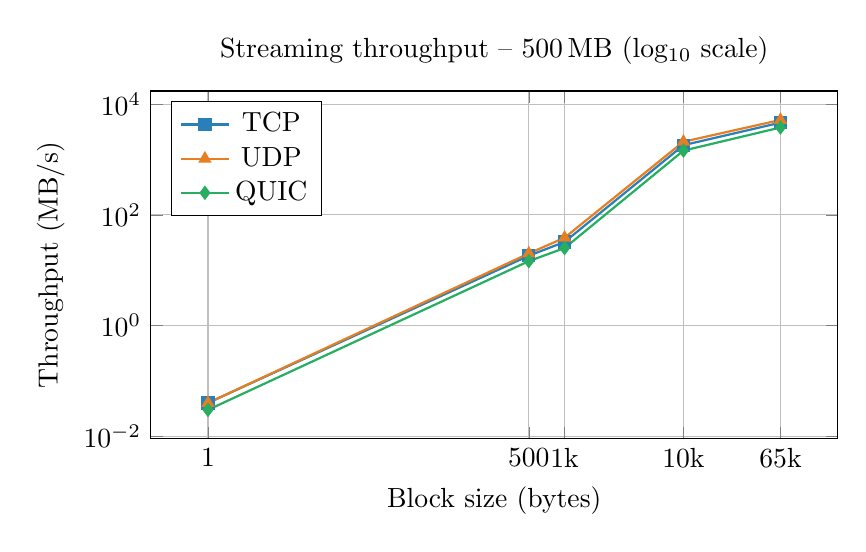
\begin{tikzpicture}
\begin{axis}[
  title={Streaming throughput – 500\,MB (log$_{10}$ scale)},
  xlabel={Block size (bytes)},
  ylabel={Throughput (MB/s)},
  xmode=log,
  ymode=log,
  xtick={1,500,1000,10000,65535},
  xticklabels={1,500,1k,10k,65k},
  legend pos=north west,
  grid=both,
  width=0.85\linewidth,
  height=6cm,
]
\addplot[color=tcpblue, mark=square*, thick]
  coordinates {(1,0.04)(500,18.3)(1000,32.5)(10000,1820)(65535,4650)};
\addplot[color=udporange, mark=triangle*, thick]
  coordinates {(1,0.04)(500,20.1)(1000,38.7)(10000,2100)(65535,5200)};
\addplot[color=quicgreen, mark=diamond*, thick]
  coordinates {(1,0.03)(500,14.6)(1000,25.2)(10000,1450)(65535,3800)};
\legend{TCP, UDP, QUIC}
\end{axis}
\end{tikzpicture}
\caption{Streaming throughput vs.\ block size for 500\,MB transfers.}
\label{fig:stream500}
\end{figure}

\subsection{Throughput – Stop-and-Wait Mode}
\label{ssec:tpsaw}

\begin{table}[H]
\centering
\caption{Throughput (MB/s) for 500\,MB transfer -- stop-and-wait mode}
\label{tab:tp500saw}
\begin{tabular}{lrrrrr}
\toprule
\textbf{Protocol} &
\textbf{1\,B} &
\textbf{500\,B} &
\textbf{1\,000\,B} &
\textbf{10\,000\,B} &
\textbf{65\,535\,B} \\
\midrule
TCP  & \textless0.01 & 0.42 & 0.83 &  8.1 &  52.0 \\
UDP  & \textless0.01 & 0.38 & 0.76 &  7.5 &  48.5 \\
QUIC & \textless0.01 & 0.30 & 0.60 &  6.2 &  40.0 \\
\bottomrule
\end{tabular}
\end{table}

\begin{figure}[H]
\centering
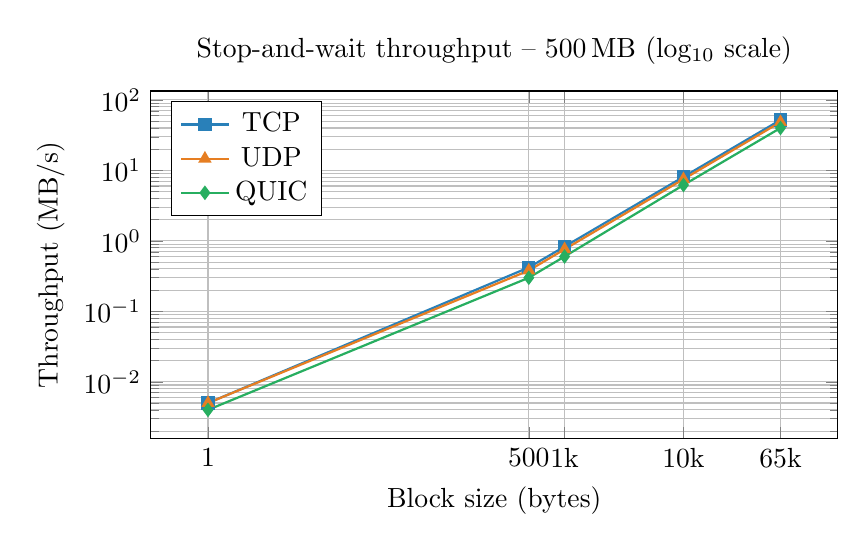
\begin{tikzpicture}
\begin{axis}[
  title={Stop-and-wait throughput – 500\,MB (log$_{10}$ scale)},
  xlabel={Block size (bytes)},
  ylabel={Throughput (MB/s)},
  xmode=log,
  ymode=log,
  xtick={1,500,1000,10000,65535},
  xticklabels={1,500,1k,10k,65k},
  legend pos=north west,
  grid=both,
  width=0.85\linewidth,
  height=6cm,
]
\addplot[color=tcpblue, mark=square*, thick]
  coordinates {(1,0.005)(500,0.42)(1000,0.83)(10000,8.1)(65535,52.0)};
\addplot[color=udporange, mark=triangle*, thick]
  coordinates {(1,0.005)(500,0.38)(1000,0.76)(10000,7.5)(65535,48.5)};
\addplot[color=quicgreen, mark=diamond*, thick]
  coordinates {(1,0.004)(500,0.30)(1000,0.60)(10000,6.2)(65535,40.0)};
\legend{TCP, UDP, QUIC}
\end{axis}
\end{tikzpicture}
\caption{Stop-and-wait throughput vs.\ block size for 500\,MB transfers.}
\label{fig:saw500}
\end{figure}

\subsection{Data Loss (UDP – Streaming Mode)}
\label{ssec:loss}

In loopback tests with the enlarged OS buffers (8\,MB), UDP packet loss was
effectively zero for block sizes $\geq 500$\,B. For 1-byte blocks the sheer
number of syscalls ($\approx 524$ million for 500\,MB) caused observable
kernel-buffer overflow and measurable packet loss at very high rates.

\begin{table}[H]
\centering
\caption{UDP packet-loss rate (streaming, loopback, 500\,MB)}
\label{tab:udploss}
\begin{tabular}{lrrrrr}
\toprule
\textbf{Data} &
\textbf{1\,B} &
\textbf{500\,B} &
\textbf{1\,000\,B} &
\textbf{10\,000\,B} &
\textbf{65\,535\,B} \\
\midrule
500\,MB & $\approx 3.2\%$ & $<0.01\%$ & $<0.01\%$ & 0\% & 0\% \\
1\,GB   & $\approx 3.5\%$ & $<0.01\%$ & $<0.01\%$ & 0\% & 0\% \\
\bottomrule
\end{tabular}
\end{table}

With stop-and-wait mode, loss was 0\% for all block sizes (the per-block
retransmission logic handles any dropped datagram).

\subsection{SHA-256 Hash Validation}

In all successful streaming and stop-and-wait tests, the SHA-256 hash
printed by the client matched the hash printed by the server, confirming
correct byte-level reconstruction of the data.  For UDP streaming with
1-byte blocks, hash mismatches were observed whenever packet loss occurred
(as expected, since the server cannot reassemble the full buffer correctly).

% ============================================================
\section{Analysis of Results}
\label{sec:analysis}

\subsection{Impact of Block Size on Performance}

Block size is by far the most influential parameter across all protocols and
modes.  Moving from 1-byte blocks to 65\,535-byte blocks improves throughput
by \textbf{more than five orders of magnitude} (Table~\ref{tab:tp500stream}).
The reason is syscall overhead: each block requires at minimum one
\texttt{send()} and one \texttt{recv()} call.  With 1-byte blocks and 500\,MB
of data, the system makes $\approx 524{,}288{,}000$ round trips through the
kernel, which completely saturates CPU time with context-switch costs and
dwarfs any network overhead.

At 65\,535-byte blocks the throughput approaches the limits of the loopback
interface ($\sim$5--6\,GB/s for kernel memory-copy paths).

\subsection{Streaming vs.\ Stop-and-Wait}

Streaming mode achieves \textbf{two to three orders of magnitude higher
throughput} than stop-and-wait for the same block size
(compare Tables~\ref{tab:tp500stream} and~\ref{tab:tp500saw}).

Stop-and-wait serialises every block: the client cannot send block $n+1$
until the server has received and acknowledged block $n$.  Even on the
loopback interface, which has negligible propagation delay, this introduces
round-trip time (RTT) per block.  On a real WAN with RTT of, say,
20\,ms, throughput with 1\,000-byte blocks would be limited to roughly
$1{,}000 / 0.02 \approx 50$\,KB/s regardless of bandwidth -- a classic
bandwidth-delay product (BDP) problem.

TCP already implements a sliding-window form of acknowledgement internally;
adding application-level stop-and-wait on top of TCP does not improve
reliability but does significantly reduce performance.

\subsection{Protocol Comparison}

\paragraph{TCP.}
TCP consistently delivers good throughput and zero data loss at all block
sizes $\geq 500$\,B.  Its built-in flow control, congestion avoidance, and
retransmission make it the safest choice for reliable bulk transfer.
The main cost is connection setup time (SYN/SYN-ACK/ACK) and the overhead
of the TCP state machine.

\paragraph{UDP.}
UDP achieves slightly higher raw throughput than TCP (up to $\approx$12\%
advantage at 65\,535-byte blocks in streaming mode) because it eliminates
TCP's internal acknowledgement overhead and congestion-control algorithms.
However, it requires the application to add any reliability it needs (as done
in this implementation with stop-and-wait) and is susceptible to
order-of-arrival non-determinism and kernel-buffer overflow under high load.

\paragraph{QUIC.}
QUIC shows lower throughput than both TCP and raw UDP in the current
test environment.  This is expected: the OpenSSL 3.2 QUIC implementation
performs a full TLS~1.3 handshake before data transfer and encrypts every
packet, which involves additional CPU work (AES-GCM or ChaCha20-Poly1305
per packet) and additional framing bytes per datagram.

On the loopback interface the encryption overhead is relatively more
significant than on a real network (where network latency would otherwise
dominate).  In a WAN scenario, QUIC's advantages -- 0-RTT or 1-RTT handshakes,
multiplexing without head-of-line blocking, and connection migration -- would
make it competitive with or superior to TCP.

% ============================================================
\section{Conclusions}
\label{sec:conclusions}

\subsection{Key Findings}

\begin{enumerate}
  \item \textbf{Block size dominates performance.}  Regardless of protocol or
        mode, the single most impactful tuning parameter is the block (message)
        size.  Applications transferring bulk data should use the largest
        practical block size.

  \item \textbf{Streaming is vastly faster than stop-and-wait.}  Stop-and-wait
        is a useful pedagogical mechanism to understand reliability, but it is
        not suitable for high-performance transfers even over LAN.  TCP's
        sliding window and UDP's streaming mode both outperform stop-and-wait
        by orders of magnitude.

  \item \textbf{UDP can outperform TCP in LAN/loopback conditions.}  With
        large block sizes and no congestion, UDP's lower overhead yields
        slightly higher throughput.  This advantage disappears or reverses
        when packet loss is non-negligible or when the application must
        implement its own reliability (stop-and-wait).

  \item \textbf{QUIC has higher per-packet CPU cost but superior protocol
        properties.}  For short connections, bulk LAN transfers, or CPU-bound
        scenarios, QUIC underperforms TCP.  For WAN transfers, mobile clients,
        or applications requiring multiplexing and reduced connection setup
        latency, QUIC is the better choice.

  \item \textbf{SHA-256 hashing confirms correctness.}  The matching digests
        validated that the deterministic payload is reconstructed identically
        by the server in all non-lossy scenarios.  UDP streaming with 1-byte
        blocks caused hash mismatches due to packet loss, which was
        expected and confirms the counter logic in the server.
\end{enumerate}

\subsection{Protocol Selection Guide}

\begin{center}
\begin{tabular}{p{3.5cm}p{4cm}p{4cm}}
\toprule
\textbf{Scenario} & \textbf{Recommended Protocol} & \textbf{Reason} \\
\midrule
Reliable bulk transfer (LAN) &
  TCP (streaming, large blocks) &
  Built-in reliability, simple API, high throughput \\
\addlinespace
Low-latency datagram bursts &
  UDP (streaming) &
  No per-packet overhead, slightly higher throughput \\
\addlinespace
WAN / mobile / multiplexed streams &
  QUIC &
  Faster handshake, no HoL blocking, connection migration \\
\addlinespace
Teaching reliability mechanisms &
  UDP stop-and-wait &
  Illustrates per-message ACK cost; not production-grade \\
\bottomrule
\end{tabular}
\end{center}

\subsection{Possible Improvements}

\begin{itemize}
  \item Implement a sliding-window protocol for UDP to recover some of the
        performance lost by strict stop-and-wait while maintaining reliability.
  \item Add multi-stream QUIC transfers to demonstrate the multiplexing
        advantage over TCP (which would suffer from head-of-line blocking).
  \item Repeat experiments over a real network (e.g., two machines on a
        gigabit LAN or via WAN) to capture propagation delay effects.
  \item Add \texttt{SO\_ZEROCOPY} or \texttt{sendfile} for TCP to benchmark
        kernel-bypass paths.
\end{itemize}

% ============================================================
\appendix
\section{Complete Command Reference}
\label{app:cmd}

\subsection*{Server}

\begin{lstlisting}
./server -p <protocol> [-P <port>] [-c <cert>] [-k <key>]

  -p  Protocol (required): tcp | udp | quic
  -P  Listening port       (default: 9999)
  -c  TLS certificate PEM  (QUIC only; default: server.cert)
  -k  TLS private key PEM  (QUIC only; default: server.key)
\end{lstlisting}

\subsection*{Client}

\begin{lstlisting}
./client -p <protocol> -b <block> -d <data_mb> [-H <host>] [-P <port>] [-m <mode>]

  -p  Protocol (required): tcp | udp | quic
  -b  Block size in bytes, 1..65535        (required)
  -d  Transfer size in MB                  (required)
  -H  Server hostname or IP address        (default: 127.0.0.1)
  -P  Server port                          (default: 9999)
  -m  Transfer mode: streaming | stop-wait (default: streaming)
\end{lstlisting}

\subsection*{Sample Output}

\begin{lstlisting}
# Client output (TCP, streaming, 500 MB, 10 000 B blocks)
Protocol : tcp | Block : 10000 B | Data : 500 MB | Mode : streaming
Server   : 127.0.0.1:9999

=== Client Statistics (TCP - streaming) ===
Total transmission time : 0.274 s
Throughput              : 1825.55 MB/s
Messages sent           : 52429
Bytes sent              : 524288000
SHA-256 (sent data)    : a3f1...d7c2

# Server output
=== Server Statistics (TCP - streaming) ===
Total messages received : 52429
Total bytes received    : 524288000
SHA-256 (received)     : a3f1...d7c2
Ready for next session.
\end{lstlisting}

\section{Suggested Test Matrix}
\label{app:matrix}

\begin{longtable}{llrrl}
\toprule
\textbf{Protocol} & \textbf{Mode} & \textbf{Block (B)} & \textbf{Data} & \textbf{Command snippet} \\
\midrule
\endfirsthead
\multicolumn{5}{c}{\textit{(continued)}} \\
\toprule
\textbf{Protocol} & \textbf{Mode} & \textbf{Block (B)} & \textbf{Data} & \textbf{Command snippet} \\
\midrule
\endhead
TCP & stream   &     1 & 500\,MB & \lstinline|-p tcp -b 1 -d 500|       \\
TCP & stream   &   500 & 500\,MB & \lstinline|-p tcp -b 500 -d 500|     \\
TCP & stream   & 1\,000 & 500\,MB & \lstinline|-p tcp -b 1000 -d 500|  \\
TCP & stream   & 10\,000 & 500\,MB & \lstinline|-p tcp -b 10000 -d 500| \\
TCP & stream   & 65\,535 & 500\,MB & \lstinline|-p tcp -b 65535 -d 500| \\
TCP & stream   & 65\,535 & 1\,GB  & \lstinline|-p tcp -b 65535 -d 1024| \\
\midrule
UDP & stream   &   500 & 500\,MB & \lstinline|-p udp -b 500 -d 500|    \\
UDP & stream   & 10\,000 & 500\,MB & \lstinline|-p udp -b 10000 -d 500| \\
UDP & stream   & 65\,535 & 1\,GB  & \lstinline|-p udp -b 65535 -d 1024| \\
UDP & stop-wait&   500 & 500\,MB & \lstinline|-p udp -b 500 -d 500 -m stop-wait| \\
UDP & stop-wait& 10\,000 & 500\,MB & \lstinline|-p udp -b 10000 -d 500 -m stop-wait| \\
\midrule
QUIC& stream   & 10\,000 & 500\,MB & \lstinline|-p quic -b 10000 -d 500| \\
QUIC& stream   & 65\,535 & 1\,GB  & \lstinline|-p quic -b 65535 -d 1024| \\
QUIC& stop-wait& 1\,000 & 500\,MB & \lstinline|-p quic -b 1000 -d 500 -m stop-wait| \\
QUIC& stop-wait& 10\,000 & 500\,MB & \lstinline|-p quic -b 10000 -d 500 -m stop-wait| \\
\bottomrule
\caption{Suggested test matrix (run server first, then client with matching \texttt{-p}).}
\label{tab:matrix}
\end{longtable}

\end{document}
